\documentclass[a4paper,10pt]{article}
\usepackage[utf8]{inputenc}
\usepackage[italian]{babel}
\usepackage{listings}
\usepackage{color}
\usepackage{subfig}
\usepackage{tikz}
\usepackage{verbatim}
\usepackage{amssymb}
\usepackage[colorlinks=true, linkcolor=black]{hyperref}
\usepackage{setspace}
%\usepackage{numprint}
%\usepackage[justification=centering]{subcaption}
\usetikzlibrary{arrows,shapes,automata,backgrounds,petri}
\usepackage{amsmath}
\usepackage{pgfplots}
\usepackage[printonlyused]{acronym}   % pacchetto per fare gli acronimi

% stile per linguaggio Matlab
\lstset{
language={Matlab},
%numbers=left,
%frame=shadowbox,
rulesepcolor=\color{black},
rulecolor=\color{black},
breaklines=true,
breakatwhitespace=true,
firstnumber=1,
firstline=1,
lastline=25,
%caption={PRISM Model V2}
xleftmargin=20pt
}


\doublespacing

\definecolor{light-gray}{gray}{0.85}
\definecolor{lbcolor}{rgb}{0.9,0.9,0.9}

\begin{document}

%\maketitle    % Creazione del Frontespizio

\begin{titlepage}
\thispagestyle{empty}
\topmargin=1cm
\large

\begin{figure}[ht]
\centering

\includegraphics[scale=0.075]{img/Stemma.jpg}
\end{figure}

\begin{center}

UNIVERSITÀ DEGLI STUDI DI FIRENZE
\vspace{0.5cm}

Laurea Magistrale in Ingegneria Informatica
\\
\normalsize
Corso di Analisi di Immagini e Video
\vspace{4cm}

\begin{huge}
Implementazione \\
Multiscale Local Binary Pattern
\end{huge}

\vspace{0.5cm}

A. Rizzo, M. Bruni

\vspace{5cm}
\rule{5cm}{.4pt}
\\
Anno accademico 2012/2013
\end{center}
\end{titlepage}

%%%%%%%%%%%%%% 

%\frontmatter % numera le pagine con numeri romani

\tableofcontents % Indice

\clearpage

\section*{Sommario}
In questa relazione, gli autori presentano un'applicazione che determina se regioni di un'immagine contengono malformazioni della tessitura al loro interno.
Verrà fatta una panoramica sulle \textit{immagini di tessiture}. Successivamente saranno presentati i concetti teorici alla base dell'operatore \textit{\acf{LBP}}. Verranno descritte delel varianti di dell'operatore \acs{LBP} base, ovvero \textit{Extended LBP}, \textit{Uniform LBP} e \textit{\acf{MLBP}}. Infine verranno mostrati gli strumenti utilizzati per lo sviluppo ed i risultati ottenuti dai test.


\newpage
\null 
\thispagestyle{empty}
\newpage


\section{Texture}

Una \textit{texture} è una nozione generale che può avere molteplici significati. In particolare nel contesto della percezione umana una texture è una specifica struttura di superfici, formate da uno o più particolari elementi, che si ripetono nello spazio.
Questa ripetizione può riguardare:

\begin{itemize}
	\item la variazione locale di scala;
	\item l'orientazione;
	\item la distribuzione spaziale dei livelli di grigio o del colore\cite{Stockman:2001:CV:558008};
	\item o altre caratteristiche geometriche dell'elemento.
\end{itemize}

\noindent In figura \ref{fig:Texture} sono rappresentati alcuni esempi di immagini di tessiture. \\

\begin{figure}[ht]
\begin{center}
\includegraphics[width=.95\textwidth]{img/Texture}
\caption{ Immagini di tessiture.}
\label{fig:Texture}
\end{center}
\end{figure}


Una immagine è percepita contenente tessiture quando il numero di elementi che la compongono è sufficientemente numeroso.
Se il numero di elementi presenti nell'immagine è ridotto, allora questi sono percepiti come un gruppo di oggetti numerabili invece che una tessitura\cite{SlidePala}.

Alcune delle caratteristiche qualitative che possono essere utilizzate per differenziare le texture sono:

\begin{itemize}
\item fineness - coarseness,
\item smoothness,
\item granularity,
\item lineation,
\item directionality,
\item regularity - randomness
\end{itemize}

\noindent L'utilizzo di modelli di tessiture può trovare interessanti applicazioni nel contesto della:

\begin{itemize}
\item Segmentazione di immagini;
\item Classificazione di immagini.
\end{itemize}

La \textit{segmentazione} di immagini consiste nel suddividerle in regioni che presentano tessiture uniformi. La \textit{classificazione}, associa ad ogni regione ottenuta dal processo di segmentazione la sua classe di appartenenza.
\section{Multi-scale Local Binary Pattern}
In questo capitolo verranno presentati alcuni concetti teorici e gli stumenti utilizzati per lo sviluppo dell'applicazione. Il primo paragrafo introdurrà il descrittore di feature \acf{LBP}. Verrà analizzata una sua variante, ovvero Uniform \acs{LBP}, che viene utilizzato per ridurre la lunghezza del vettore di feature. Analizzeremo infine la sua estensione \acf{MLBP}.

\subsection{Local Binary Pattern}

\acf{LBP} è un efficiente texture operator, introdotto per la prima volta nel 1994 \cite{LBPfirst}. Le feature estratte con questo metodo vengono utilizzate per la classificazione di immagini in ambito della computer vision.
\acs{LBP} associa ai pixel dell'immagine un'etichetta, determinata tramite un'operazione di confronto tra il pixel in esame ed un certo numero di pixel nelle sue vicinanze, \emph{neighborhood}.
Tra le caratteristiche principali di \acs{LBP} troviamo:

\begin{itemize}
	\item è robusto alla variazione uniforme dell'illuminazione dell'immagine;
	\item è robusto al rumore;
	\item non è invariante alle rotazioni dell'immagine;
	\item non è invariante alla scala.
\end{itemize}

Un altra importante proprietà è infine la sua semplicità computazionale che lo rende ideale per l'analisi delle immagine in \acf{RT}.

\subsubsection{Descrizione}

L'idea alla base dell'operatore \acf{LBP} è che le texture bidimensionali possono essere descritte attraverso pattern locali.
L'implementazione base dell'operatore \acs{LBP} etichetta i pixel dell'immagine attraverso un'operazione di sogliatura dei pixel contenuti in una maschera 3 x 3.

 Il pixel centrale viene confrontato con ogni vicino ed il risultato del confronto viene espresso con un numero binario.\\

\begin{figure}[ht]
\begin{center}
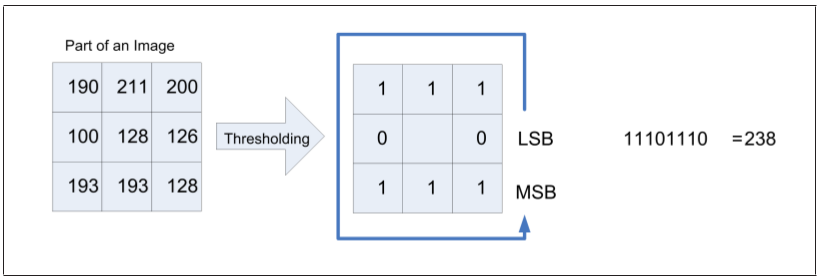
\includegraphics[width=.95\textwidth]{img/LBP_code}
\caption{ Estrazione del codice LBP.}
\label{fig:LBPcode}
\end{center}
\end{figure}

Riferendoci alla figura \ref{fig:LBPcode} il processo di etichettatura dei pixel è il seguente. Il livello di grigio del pixel centrale, detto anche \emph{pivot} viene confrontato con il livello di grigio di tutti gli altri pixel della maschera che viene binarizzata attraverso la seguente funzione:

\begin{equation}
s(x) = 	\begin{cases} 1, & \mbox{se } x \ge 0 \\ 0, & \mbox{se } x < 0 \end{cases}
\end{equation}

dove $x$ è la differenza tra l'intensità del livello di grigio di un pixel del \emph{neighborhood} ed il livello di grigio del pixel pivot. I valori così ottenuti vengono concatenati in senso antiorario andando a formare un codice binario di 8 bit la cui conversione decimale rappresenta il codice \acs{LBP} del pixel pivot.

\subsubsection*{Descrittore}
Il numero totale di codici \acs{LBP} è pari a $2^8 = 256$.
L'istogramma dei codici LBP calcolati sui pixel dell'immagine può essere utilizzato come descrittore della texture. In figura \ref{fig:istCompleteLBP} è mostrato l'istogramma di un immagine LBP.

\begin{figure}[ht]
\begin{center}
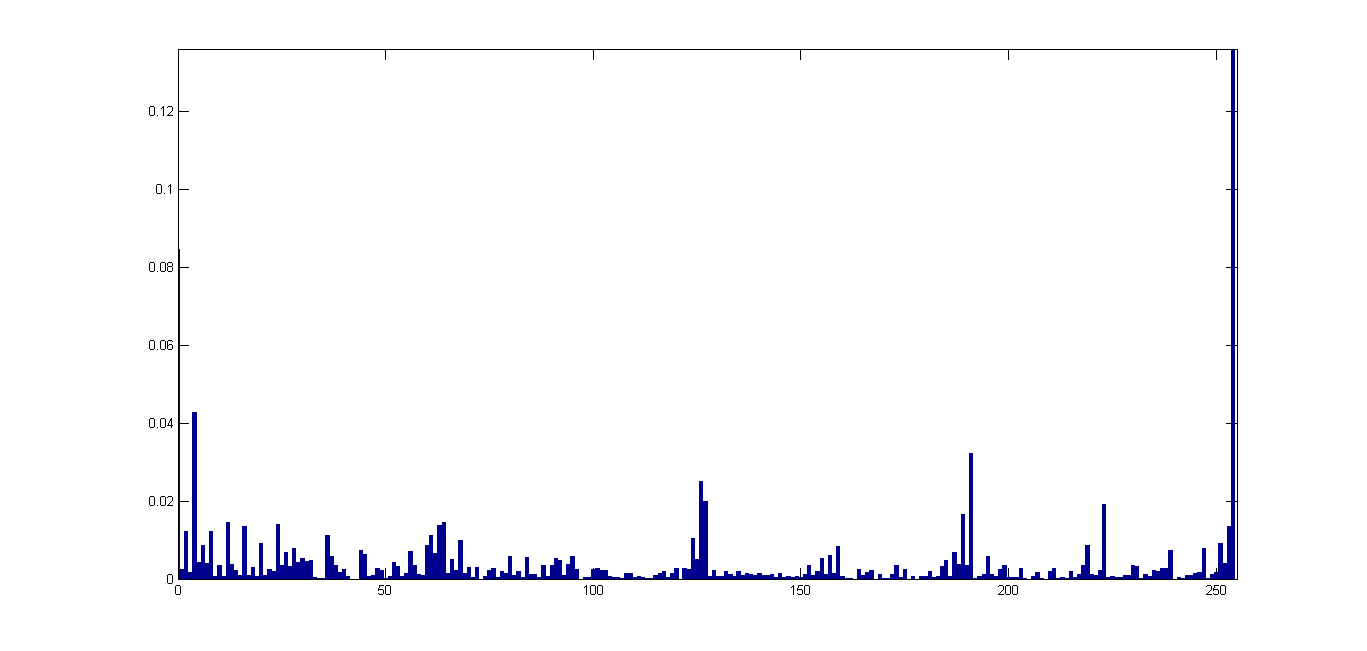
\includegraphics[width=.95\textwidth]{img/hist-complete}
\caption{ Istogramma normalizzato di un'immagine LBP. }
\label{fig:istCompleteLBP}
\end{center}
\end{figure}

Per il calcolo dell'istogramma si utilizza la seguente formula:

\begin{equation}
h(i) = \sum_{x,y} B(LBP_{P,R}(x, y)) = i, i \in  [0, 2^P-1 ]
\end{equation}

dove

\begin{equation}
B(v) = 	\begin{cases} 1, & \mbox{v = true} \\ 0, & \mbox{altrimenti} \end{cases}
\end{equation}

\subsection{Extended LBP}
Finora abbiamo considerato come neighborhood i pixel adiacenti a quello di pivot. Una variante dell'operatore \acs{LBP} è l' \acf{ELBP} o \acf{CLBP} . \acs{ELBP} considera come neighborhood i $P$ pixel che si trovano ad una distanza $R$ dal pivot. Le coordinate dei $P$ pixel si possono ottenere con la seguente formula:

\begin{equation}
(x_p, y_p) = ( - Rsin( \frac{2\pi p}{P} ), Rcos( \frac{2\pi p}{P} ) )  , \quad p = 0, \cdots, P-1
\end{equation}

Nel caso in cui le coordinate ottenute non corrispondono alla griglia discreta dell'immagine si effettua una interpolazione bilineare.

In figura \ref{fig:NeighborhoodLBP} sono mostrati alcuni risultati dell'applicazione della formula appena descritta.

\begin{figure}[ht]
\begin{center}
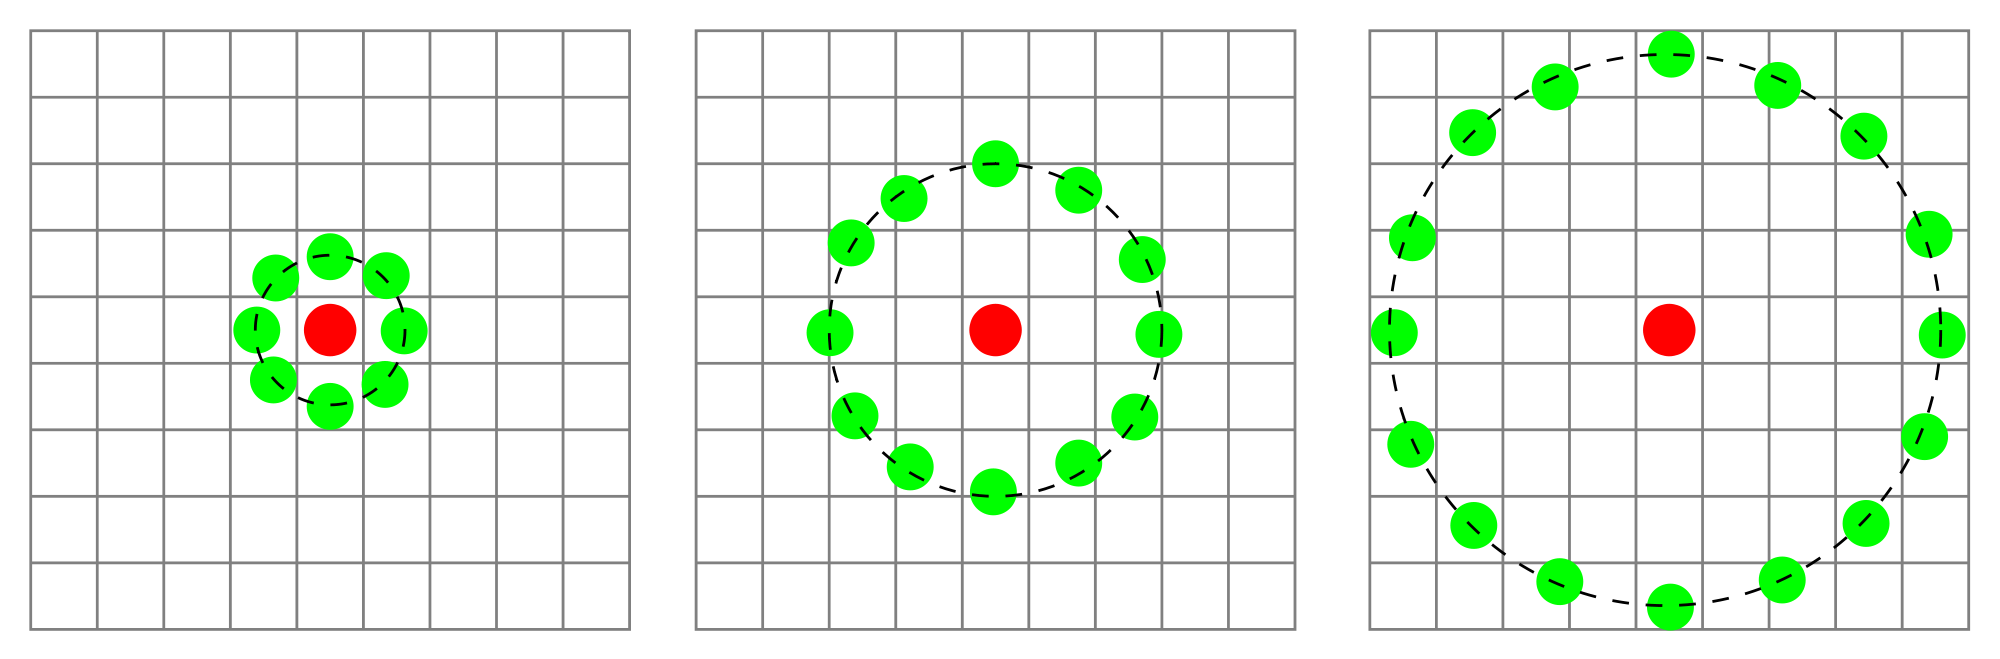
\includegraphics[width=.95\textwidth]{img/raggio_LBP}
\caption{ Neighborhood per il calcolo del codice LBP nei casi: $(P=8, R=1)$, $(P=12, R=2)$ e $(P=16, R=4)$. }
\label{fig:NeighborhoodLBP}
\end{center}
\end{figure}


La formula seguente permette di calcolare, in base dieci, il codice LBP di lunghezza $P$ e raggio $R$ generico di un pixel.

\begin{equation}
LBP_{P,R}(x, y) = \sum_{p=0}^{P-1}{s(g_p - g_c)2^p}
\end{equation}

\subsection{Uniform Local Binary Pattern}
Come accennato precedentemente l'istogramma dell'immagine LBP è utilizzato come descrittore della texture. Utilizzando l'operatore LBP base, otteniamo un istogramma con $256$ classi. Per ridurre la dimensione del descrittore si può utilizzare Uniform \acf{LBP}. Uniform \acs{LBP} considera solo i pattern in cui occorrono al più due transizioni da $0$ a $1$ o da $1$ a $0$ tra pixel adiacenti. Per esempio:

\begin{itemize}
	\item $00000000 \rightarrow 0$ transizioni
	\item $01110000 \rightarrow 2$ transizioni
	\item $11001111 \rightarrow 2$ transizioni
	\item $11001001 \rightarrow 4$ transizioni
	\item $01010010 \rightarrow 6$ transizioni
\end{itemize}

I pattern che soddisfano le condizioni di Uniform \acs{LBP} sono in totale $58$, come mostrato in figura \ref{fig:uniformLBP}.

\begin{figure}[ht]
\begin{center}
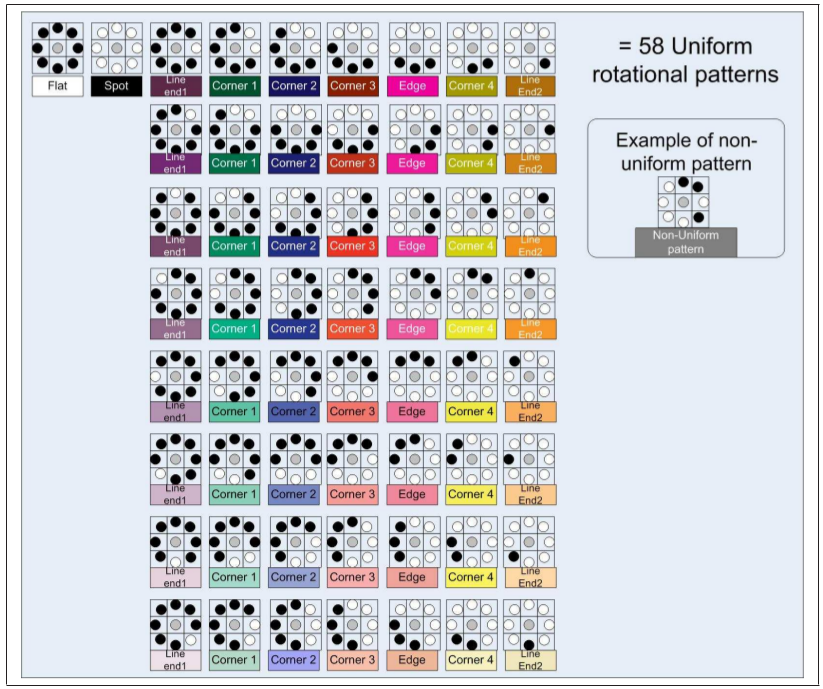
\includegraphics[width=.95\textwidth]{img/uniform_LBP}
\caption{ Pattern di Uniform LBP.}
\label{fig:uniformLBP}
\end{center}
\end{figure}

Questa variante si basa sul fatto che le feature così estratte sono più robuste al rumore e l'istogramma risultante è di dimensione inferiore mantenendo comunque le feature rilevanti.

In figura \ref{fig:istUniformLBP} è mostrato l'istogramma di un immagine su cui è stato applicato l'operatore di Uniform \acs{LBP}.

\begin{figure}[ht]
\begin{center}
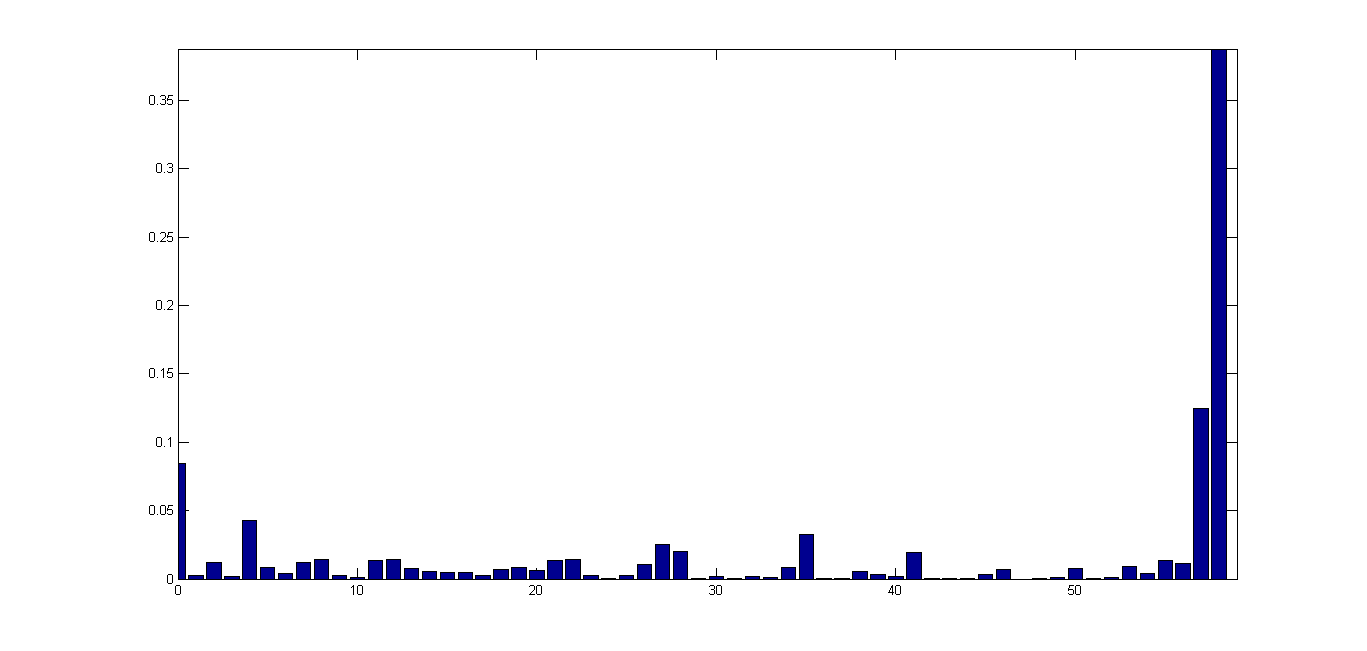
\includegraphics[width=.95\textwidth]{img/hist-uniform}
\caption{ Istogramma normalizzato di una immagine su cui è stato applicato l'operatore di Uniform \acs{LBP}. I primi $58$ pattern sono quelli uniformi, mentre l'ultimo pattern corrisponde a tutti i pixel con codice non uniforme.}
\label{fig:istUniformLBP}
\end{center}
\end{figure}

Per ottenere il codice di Uniform \acs{LBP} si utilizza la formula seguente:

\begin{equation}
LBP_{P,R}^{u2}(x, y)=	
\begin{cases} 
I(LBP_{P,R}(x, y)), & \mbox{se } U(LBP_{P,R}) \le 2, I(z) \in [0, (P-1)P+2 )   \\
(P-1)P+2, & \mbox{altrimenti}
\end{cases}
\end{equation}

dove la funzione $U(x)$ calcola il numero di transizioni.

\begin{equation}
U(LBP_{P,R}) = |s( g_{P-1} - g_{c}) - s(g_{0} - g_{c}) | + \sum_{p = 1}^{P} |s(g_{p} - g_{c}) - s( g_{P-1} - g_{c}) |
\end{equation}

\subsection{Multiscale Local Binary Pattern}
\acf{MLBP} è un'estensione dell'operatore \acs{LBP}. \acs{MLBP} è ottenuto combinando i descrittori delle texture ottenuti facendo variare il raggio $r \in [r_min, R]$ per la determinazione dei neighbor. 
Alternativamente \acs{MLBP} può essere ottenuto applicando l'operatore \acs{LBP} con raggio costante su l'immagine a risoluzione ridotta. Quest'ultimo metodo è meno efficace in quanto riducendo la risoluzione dell'immagine risulta più difficile estrarre informazioni sul contrasto tra piccole regioni lontane fra loro.

Le feature estratte con \acs{MLBP} risultano migliori rispetto a \acs{LBP} per la classificazione di immagini.

\subsubsection{Descrittore}
Il descrittore della texture ottenuto con \acs{MLBP} è la concatenazione degli istogrammi ottenuti applicando iterativamente \acs{LBP} sulla stessa immagine al variare del raggio $r \in \left\lbrace  r_1, r_2, \cdots, r_R \right\rbrace$. Il descrittore è dato dalla seguente formula:

\begin{equation}
f = [h_{P, r_{1}}, h_{P, r_{2}}, \cdots, h_{P, r_R}]
\end{equation}

\noindent dove

\begin{equation}
h_{P,r}(i) = \sum_{x, y} B(LBP_{P,r}(x, y)) = i, i \in  [0, L-1 ], r \in \left\lbrace  r_1, r_2, \cdots, r_R \right\rbrace
\end{equation}

\noindent con $L$ numero massimo di classi dell'istogramma e

\begin{equation}
B(v) = 	\begin{cases} 1, & \mbox{v = true} \\ 0, & \mbox{altrimenti} \end{cases}
\end{equation}

\subsection{Filtro di smoothing gaussiano}
I filtri di \emph{smoothing} vengono utilizzati principalmente per ridurre il rumore presente nell'immagine. Sono anche detti \emph{filtri di media}. Infatti facendo scorrere lungo l'immagine la maschera del filtro, detta anche \emph{kernel mask}, il valore di ogni pixel viene sostituito con la media pesata dei livelli di grigio dei pixel interni alla regione della maschera. Il processo di smoothing permette di ridurre i dettagli meno significativi dell'immagine e mettere in risalto le caratteristiche strutturali della stessa.
Un effetto indesiderato dello smoothing è quello di produrre un'immagine sfocata, soprattutto se applicato iterativamente.
La figura \ref{fig:kernelMask} mostra un filtro di smoothing generico 3x3. La maschera del filtro verrà moltiplicata per un coefficiente di normalizzazione in modo tale che la somma degli elementi della mascherà sia uno. I coefficienti della maschera vengono scelti secondo il seguente principio: il peso associato al pixel centrale assume un valore superiore rispetto agli altri. I pesi associati agli altri pixel assumono valori decrescenti all'aumentare della distanza dal pixel centrale. In altre parole si vuole fare in modo che il pixel centrale abbia una maggiore importanza nel calcolo della media. Viceversa i pixel più lontani da quello centrale peseranno di meno nel calcolo della media. Questo permette di ridurre l'effetto indesiderato del processo di smoothing.

\begin{figure}[ht]
\begin{center}
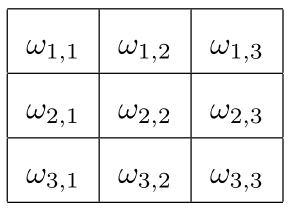
\includegraphics[width=.3\textwidth]{img/kernel_mask}
\caption{ Esempio di una kernel mask di dimensioni 3x3, dove $\omega_{i,j}$ reppresenta il peso applicato al valore del livello di grigio del corrispettivo pixel nell'immagine}
\label{fig:kernelMask}
\end{center}
\end{figure}

I coefficienti della maschera sono calcolati utilizzando la \emph{2D Gaussian Smoothing Operator} $G(x,y)$, cui formula è riportata qui di seguito:

\begin{equation}
G(x, y) = e^{- \frac{(x^2 + y^2)}{2\sigma^2}}
\end{equation}

La dimensione $n$ della kernel mask è legata al valore di $\sigma$ dalla seguente formula:

\begin{equation}
6\sigma - 1 = n
\end{equation}

%\begin{center}
%\begin{tabular}[ht]{|c|c|c|}\hline
%	$\omega_{1,1}$ & $\omega_{1,2}$ & $\omega_{1,3}$ \\ \hline
%	$\omega_{2,1}$ & $\omega_{2,2}$ & $\omega_{2,3}$ \\ \hline
%	$\omega_{3,1}$ & $\omega_{3,2}$ & $\omega_{3,3}$ \\ \hline
%\end{tabular}
%\end{center}
\section{Implementazione}
In questo capitolo verranno illustrati gli strumenti e gli algoritmi utilizzati per l'implementazione del software.

\subsection{Strumenti}
Per lo studio e l'implementazione del \acf{MLBP} è stata creata una libreria in Matlab. 
Matlab (MATrix LABoratory) è un ambiente per il calcolo numerico e l'analisi statistica che comprende anche l'omonimo linguaggio di programmazione creato dalla MathWorks \cite{MATLAB:2013}.

La libreria creata è stata utilizzata in un'applicazione per la rilevazione di errori all'interno di immagini di tessiture.
Per permettere un uso agevole del software e della configurazione dei parametri è stata sviluppata una \acf{GUI}, mostrata in figura \ref{fig:GUI}.
I dati inseriti all'interno dei campi di input devono rispettare la sintassi del linguaggio Matlab. Ad esempio per i campi \textit{radii} e \textit{training set}, in cui è possibile inserire un array di valori, è accettata la seguente sintassi:

\begin{lstlisting}
inizio:step:fine [, inizio2:step2:fine2]
\end{lstlisting}

ad esempio se si vuole ottenere un array con i valori: $1, 3, 5, 7 $, basterà scrivere: $1:2:7$.

Il codice sorgete di tutta l'applicazione è disponibile sul servizio di versioning Github (\href{http://dining-engineers.github.io/Multi-scale-Local-Binary-Pattern/}{http://dining-engineers.github.io/Multi-scale-Local-Binary-Pattern/}).\\

\begin{figure}[ht]
\begin{center}
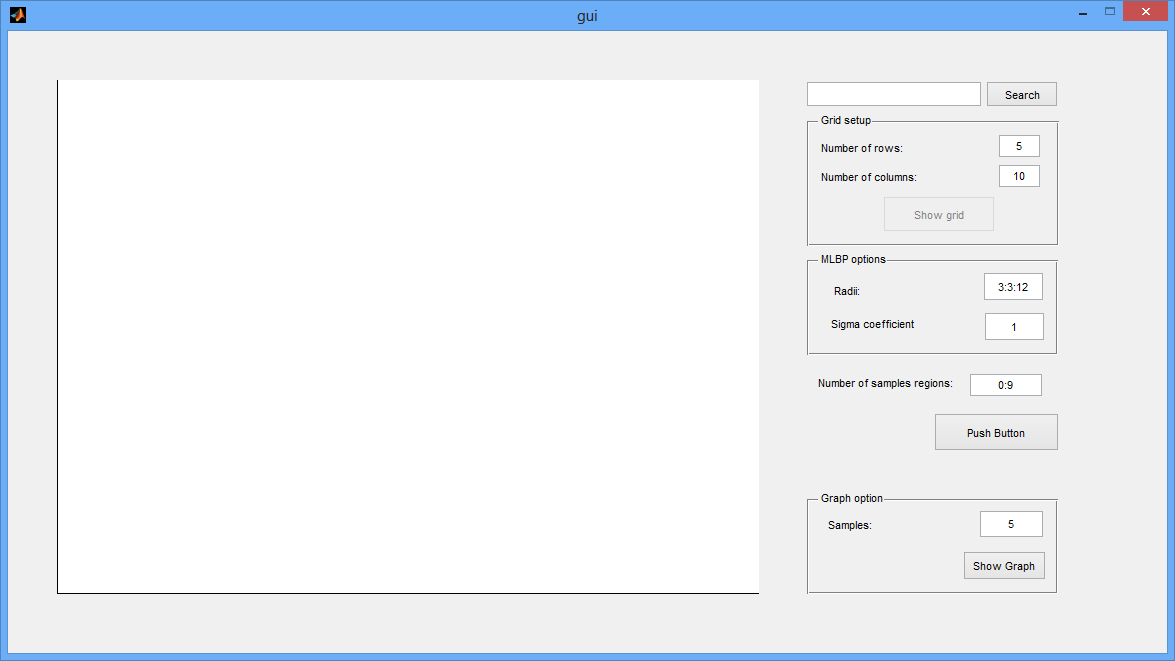
\includegraphics[width=.95\textwidth]{img/gui}
\caption{GUI.}
\label{fig:GUI}
\end{center}
\end{figure}

\pagebreak

Le directory sono organizzate nel modo seguente:

\begin{itemize}
	\item \textit{Dataset}: contiene le immagini del dataset;
	\item \textit{Documents}: contiene tutti i documenti consultati per lo sviluppo dell'applicazione. In particolare, nella sottodirectory \textit{relazione} sono contenuti i sorgenti LaTeX della relazione del il file PDF della stessa;
	\item \textit{src}: contiene il codice sorgente dell'applicazione.
\end{itemize}

L'organizzazione delle directory è raffigurata nella figura \ref{fig:orgDir}

\begin{figure}[ht]
\begin{center}
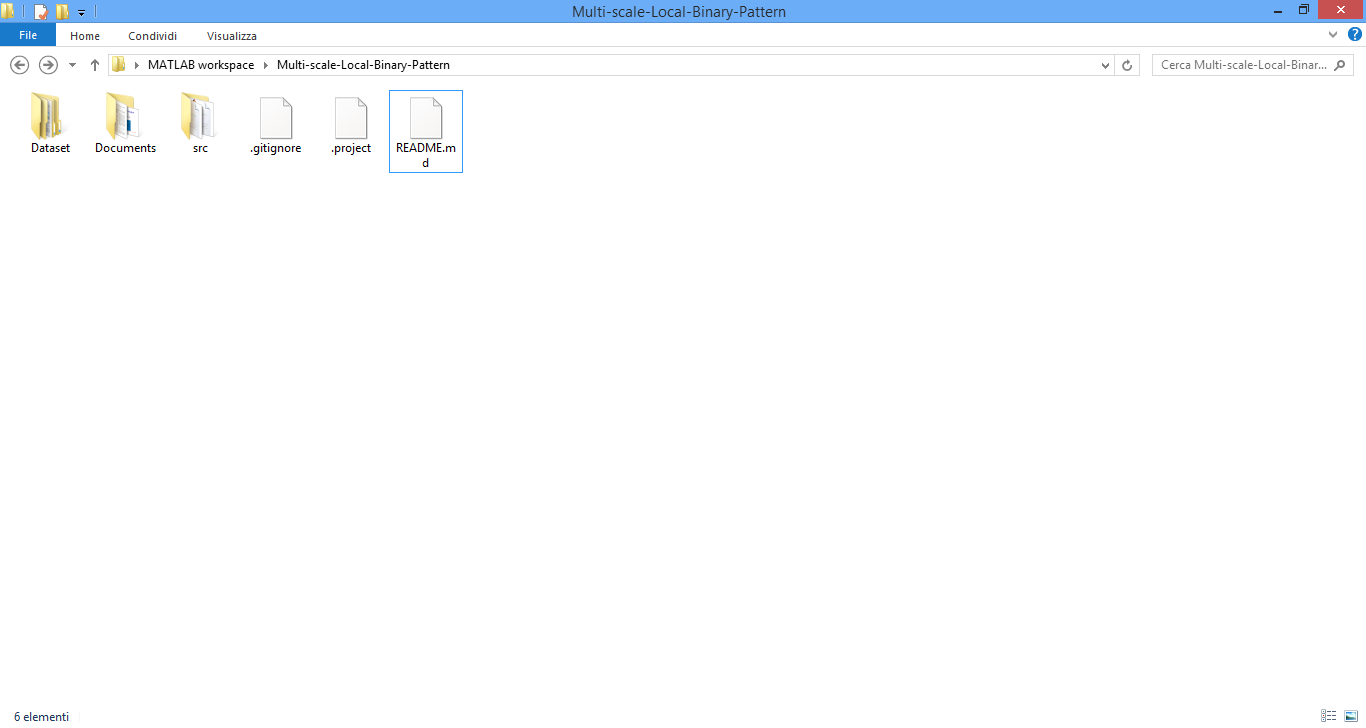
\includegraphics[width=.95\textwidth]{img/organizzazione_Cartelle}
\caption{Organizzazione delle directory dell'applicazione.}
\label{fig:orgDir}
\end{center}
\end{figure}

\pagebreak

\subsection{Analisi dell'immagine}
\label{imp:analisi}
Nel contesto della nostra applicazione, le immagini in esame saranno analizzate in scala di grigio.
Per ottenere un descrittore della texture dell'immagine è stata implementata la funzione

\begin{lstlisting}
function [ descriptor ] = getMLBPDescriptor( img, mapping, radii, num_region_rows, num_region_cols, sigma_coefficient )
\end{lstlisting}

che richiede in input: l'immagine da elaborare, la variante di \acs{LBP} da utilizzare (nel nostro caso Uniform LBP), un array contenente i raggi per fare \acs{MLBP}, il numero di righe e colonne in cui l'immagine verrà suddivisa ( paragrafo \ref{imp:seg}) ed infine il valore della deviazione standard per l'applicazione del filtro di smoothing gaussiano.

Al suo interno, getMLBPDescriptor(), applica iterativamente all'immagine l'operatore \acs{LBP}.
Ad ogni iterazione $i$, all'immagine viene inizialmente applicato il filtro di smoothing gaussiano

\begin{lstlisting}
% apply gauss smoothing
myfilter = fspecial( 'gaussian', kernel_size, sigma_coefficient );
img = imfilter( img, myfilter, 'replicate' );
\end{lstlisting}

\noindent Successivamente viene chiamata la funzione\cite{lbpcode}

\begin{lstlisting}
function [lbp_img] = lbp( img, radius, num_neighbors, mapping );
\end{lstlisting}

\noindent che calcola l'immagine \acs{LBP} con raggio $radii(i)$, (paragrafo \ref{MLBP:extended}).

\subsubsection{Suddivisione dell'immagine in regioni}
\label{imp:seg}
Al fine di determinare le regioni della tessitura in cui sono presenti degli errori, abbiamo deciso di suddividere l'immagine in regioni non sovrapposte. I parametri $num\_region\_rows$ e $num\_region\_cols$ determinano il numero di regioni in cui l'immagine viene suddivisa.
Le regioni sono numerate da $0$ a $num\_region\_rows \cdot num\_region\_cols - 1$.
Le coordinate della k-esima regione sono ottenute attraverso l'utilizzo della funzione

\begin{lstlisting}
function [ rMin, rMax, cMin, cMax ] = gridBounds( imgSize, num_region_rows, num_region_cols, k )
\end{lstlisting}

In figura \ref{fig:GUIpreLBP} viene mostrata la suddivisione in regioni dell'immagine di input. \\

\begin{figure}[ht]
\begin{center}
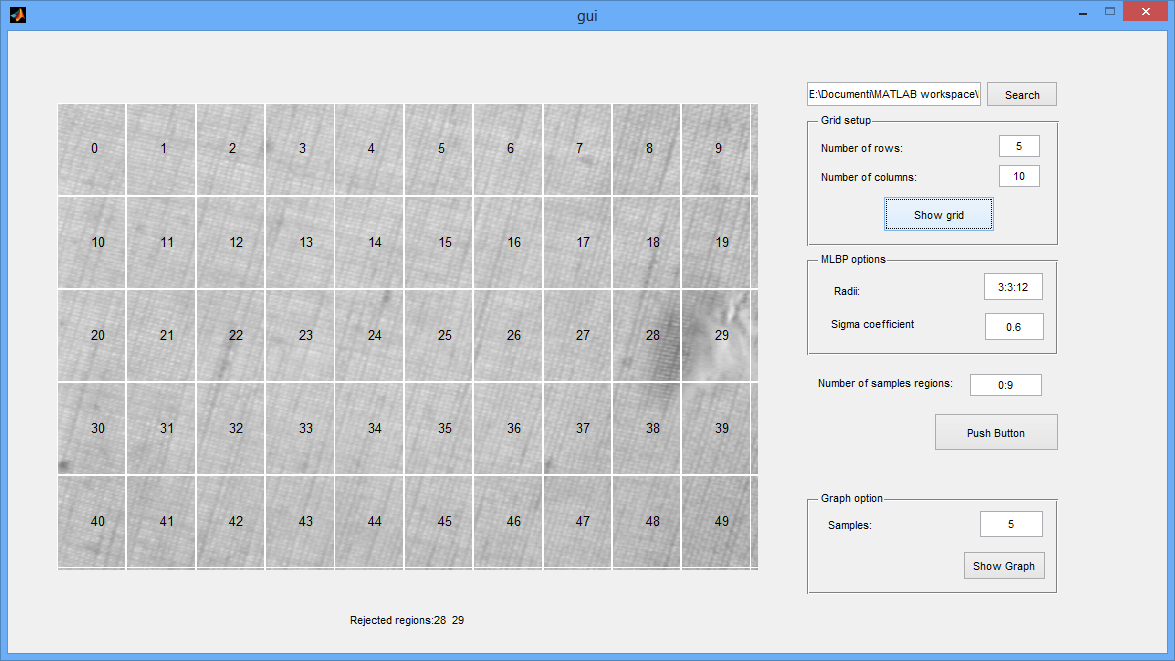
\includegraphics[width=.95\textwidth]{img/gui_pre_lbp}
\caption{ Screenshot della GUI in cui viene mostrata la suddivisione in regioni dell'immagine di input.}
\label{fig:GUIpreLBP}
\end{center}
\end{figure}

In seguito all'operazione di segmentazione dell'immagine, per ogni regione, viene estratto il relativo descrittore \acs{MLBP}:

\begin{equation*}
f = [h_{P, r_{1}}, h_{P, r_{2}}, \cdots, h_{P, r_R}]
\end{equation*}


\noindent come spiegato nel paragrafo \ref{mlbp:desc-mlbp}. 



%	\pagebreak 
%	
%	La costruzione dell'istogramma associato all'LBP di raggio r, $h_{P,r}$ è ottenuta nel modo seguente:
	
%	\begin{lstlisting}
%	M = lbp_image(rMin:rMax, cMin:cMax );
%	% compute histogram of subregion M
%	h = hist(M(:),0:(mapping.num-1));
%	% normalizie histogram
%	h = h/sum(h);
%	\end{lstlisting}



\subsection{Misura di similarità}

Per misurare la similarità tra i descrittori di due regioni $I$ e $J$, possono essere utilizzati vari criteri. Abbiamo implementato le seguenti misure di similarità $Sim(I, J)$:

\begin{itemize}

\item Chi-square criterion:
\begin{equation}
Sim(I, J) = -  \sum_{i} \frac{ (f_{I}(i) - f_{J}(i) )^2}{f_{I}(i) + f_{J}(i)}
\end{equation}

\item Histogram intersection:
\begin{equation}
Sim(I, J) = \sum_{i} \mbox{min}(f_{I}(i),f_{J}(i))
\end{equation}

\item Log-likelihood ratio (Kullack-Leibler 
divergence):
\begin{equation}
Sim(I, J) = - \sum_{i} f_{I}(i)log(f_{J}(i)
\end{equation}

\item Normalize Correlation:
\begin{equation}
Sim(I, J) = \frac{f_{I}f_{J}'}{||f_{I}|| ||f_{J}||}
\end{equation}

\item Normalize Cross-correlation:
\begin{equation}
Sim(I, J) = \frac{\sigma_{f_{I}f_{J}}}{\sigma_{f_{I}}\sigma_{f_{J}}}
\end{equation}


\end{itemize}

Tra le misure sopra descritte, è stato scelto di utilizzare la misura di similarità \textit{Normalize Correlation}. Nel caso in cui l'utente preferisca utilizzare un'altra misura di similarità è sufficiente modificare il codice nella funzione \textit{computeRejectedRegions}, dove viene specificata la misura di similarità in uso.



\pagebreak
\subsection{Testing}

Lo scopo dell'applicazione è quello di determinare se alcune regioni presentano malformazioni della tessitura al loro interno. Per poter classificare una regione come corretta o errata, è necessario conoscere un certo numero di regioni sicuramente corrette. Come possiamo vedere in figura \ref{fig:GUIpostLBP}, l'utente può specificare nel campo \textit{number of samples regions} il numero delle regioni esatte che vanno a definire il \textit{training set}.

Ogni regione corretta viene confrontata con tutte le altre regioni del training set utilizzando la misura di similarità $Sim(I, J)$, dove  $I$ e $J$ rappresentano i descrittori \acs{MLBP}.
In questo modo si ottengono le misure di similarità del training set da cui possiamo estrarre un valore medio ($\mu_{training}$) ed una deviazione standard ($\sigma_{training}$) che definiscono una distribuzione gaussiana delle misure di similarità delle regioni corrette.

Per classificare una regione $k$, che non appartiene al training set, si confronta il suo descrittore con tutti i descrittori del training set utilizzando la medesima misura di similarità $Sim(I, J)$. In questo modo si ottengono le misure di similarità della regione di test con il training set da cui possiamo estrarre un valore medio ($\mu_{test}$) ed una deviazione standard ($\sigma_{test}$).

La regione $k$ verrà classificata come corretta se rispetta la seguente condizione:

\begin{equation}
|\mu_{training}- \mu_{test}| \le 3\sigma_{training}
\end{equation}

\noindent altrimenti verrà classificata come una regione contenente difetti.

\pagebreak

\subsubsection{Dataset}
Il \textit{dataset} utilizzato per testare l'applicazione consiste in un insieme di immagini che raffigurano la trama di tessuti. All'interno di alcune di queste immagini sono presenti uno o più difetti che la procedura dovrà identificare. In figura \ref{fig:esDataset} sono rappresentate alcune immagini del dataset.

\begin{figure}[ht]
\begin{center}
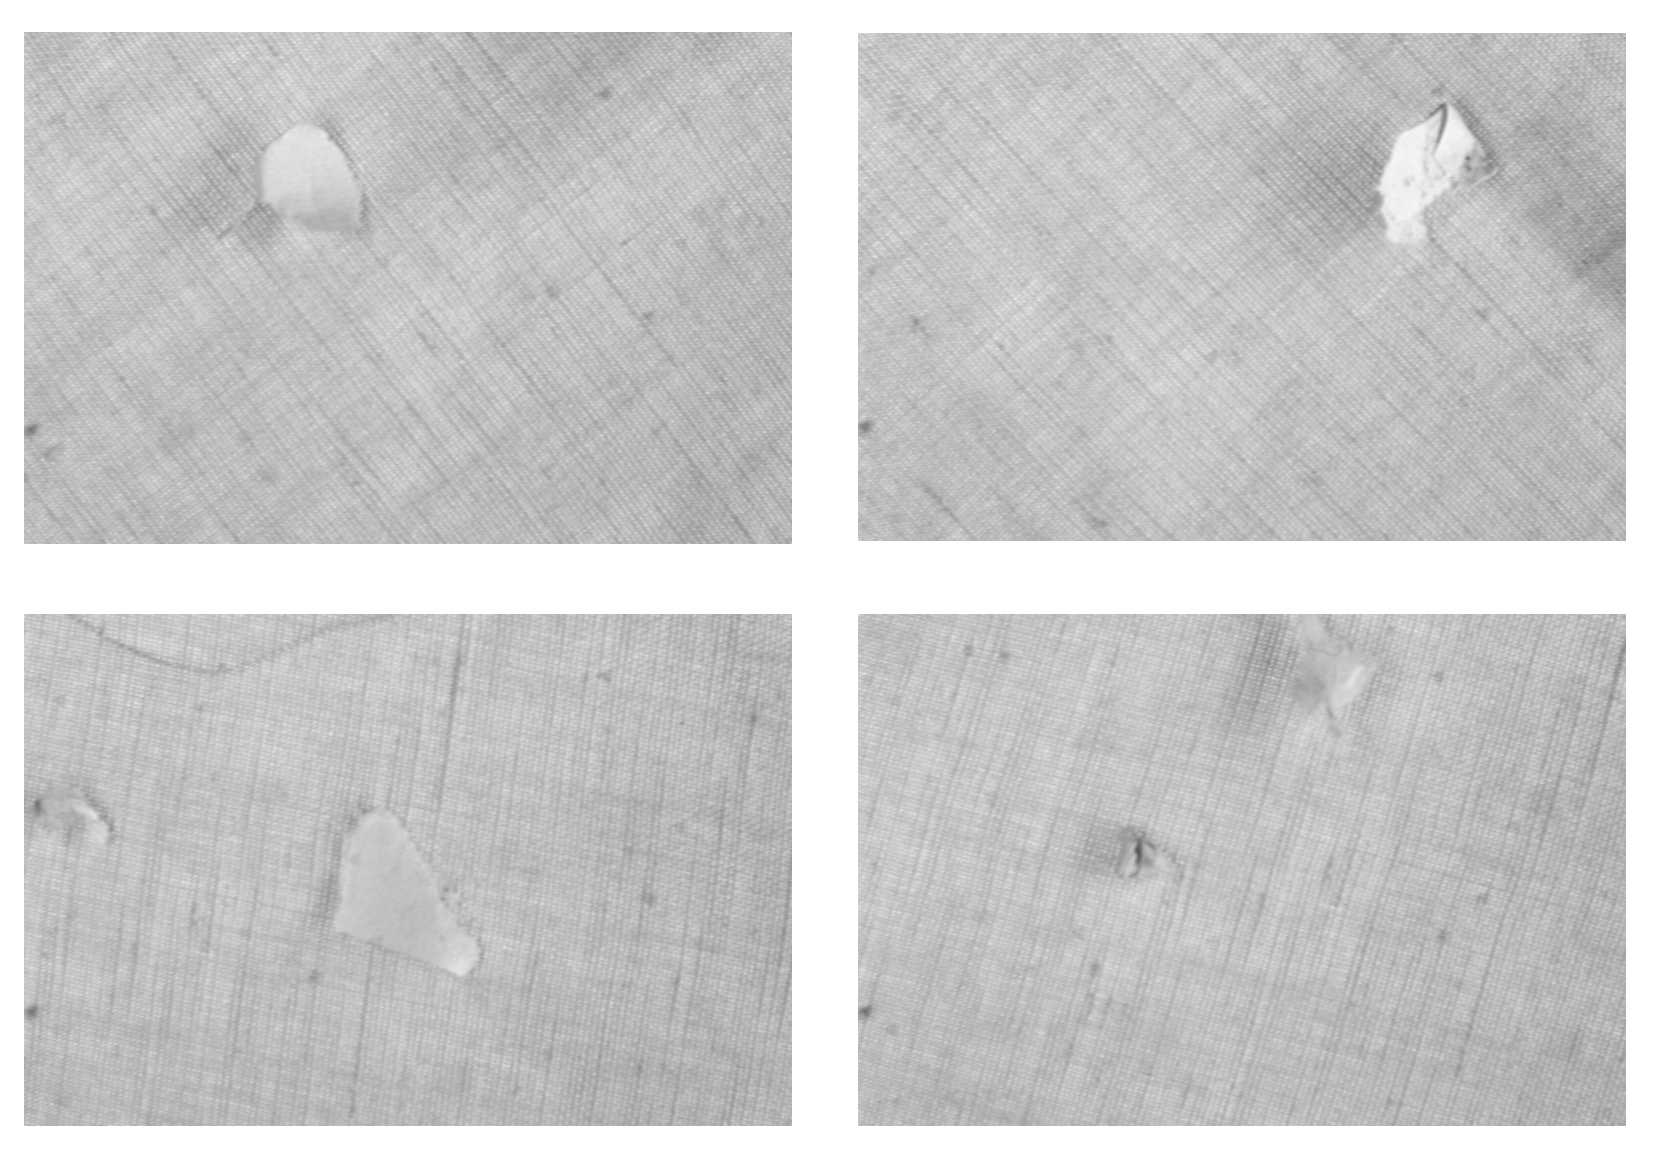
\includegraphics[width=.95\textwidth]{img/esempioDataset}
\caption{ Esempio di immagini utilizzate nel dataset.}
\label{fig:esDataset}
\end{center}
\end{figure}

\pagebreak

\subsection{Risultati e conclusioni}
Applicando la regola di classificazione descritta nel paragrafo precedente, ogni regione viene classificata ed i risultati vengono riportati direttamente sull'immagine come mostrato nella figura \ref{fig:GUIpostLBP}.

\begin{figure}[ht]
\begin{center}
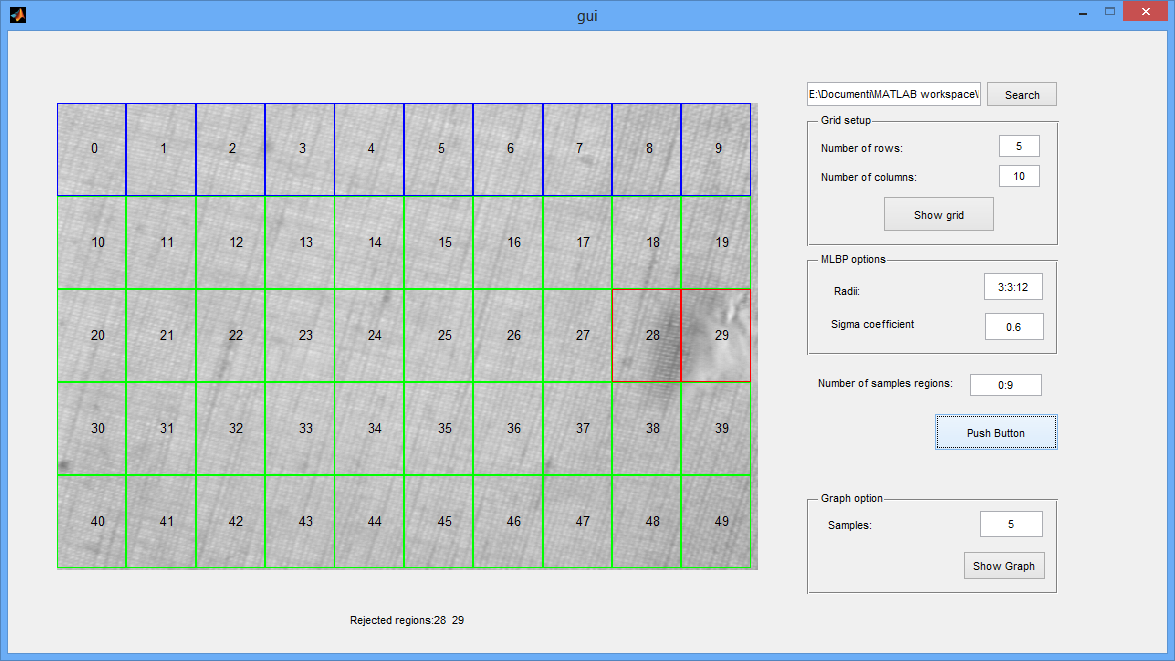
\includegraphics[width=.95\textwidth]{img/gui_post_lbp}
\caption{Risultati dell'operazione di classificazione. Le regioni con contorno di colore rosso sono quelle contenenti difetti, le regioni di colore blu sono quelle del training set e le regioni con contorno verde sono quelle ritenute corrette. }
\label{fig:GUIpostLBP}
\end{center}
\end{figure}

L'utente, cliccando sull'apposito bottone \textit{Show Graph}, può visualizzare i grafici delle distribuzioni gaussiane determinate precedentemente. In figura \ref{fig:worstGraph} è visualizzato un esempio dei grafici delle distribuzioni gaussiane delle cinque regioni con media $\mu_{test}$ peggiori.


\begin{figure}[ht]
\begin{center}
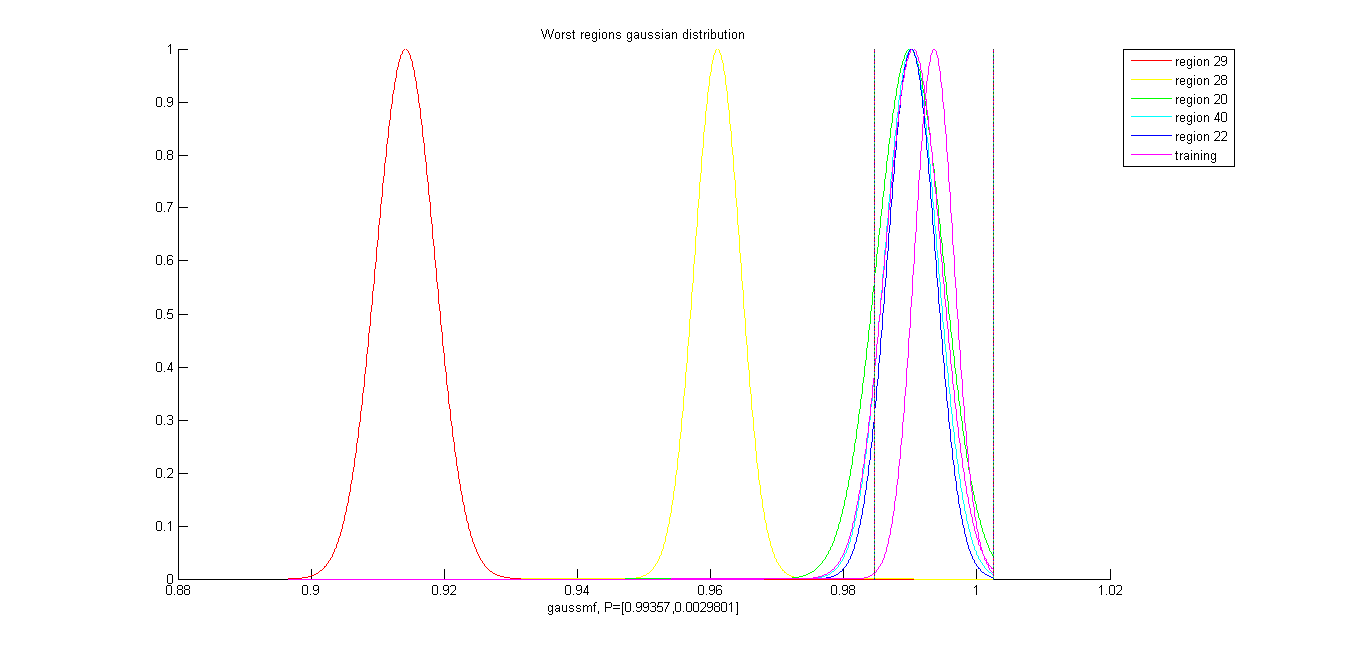
\includegraphics[width=1\textwidth]{img/worst_graph}
\caption{ Caso peggiore }
\label{fig:worstGraph}
\end{center}
\end{figure}


In figura \ref{fig:worstBestGraph}, è visualizzato un esempio dei grafici delle distribuzioni gaussiane delle cinque regioni con media $\mu_{test}$ peggiori tra quelle classificate come regioni corrette.


\begin{figure}[ht]
\begin{center}
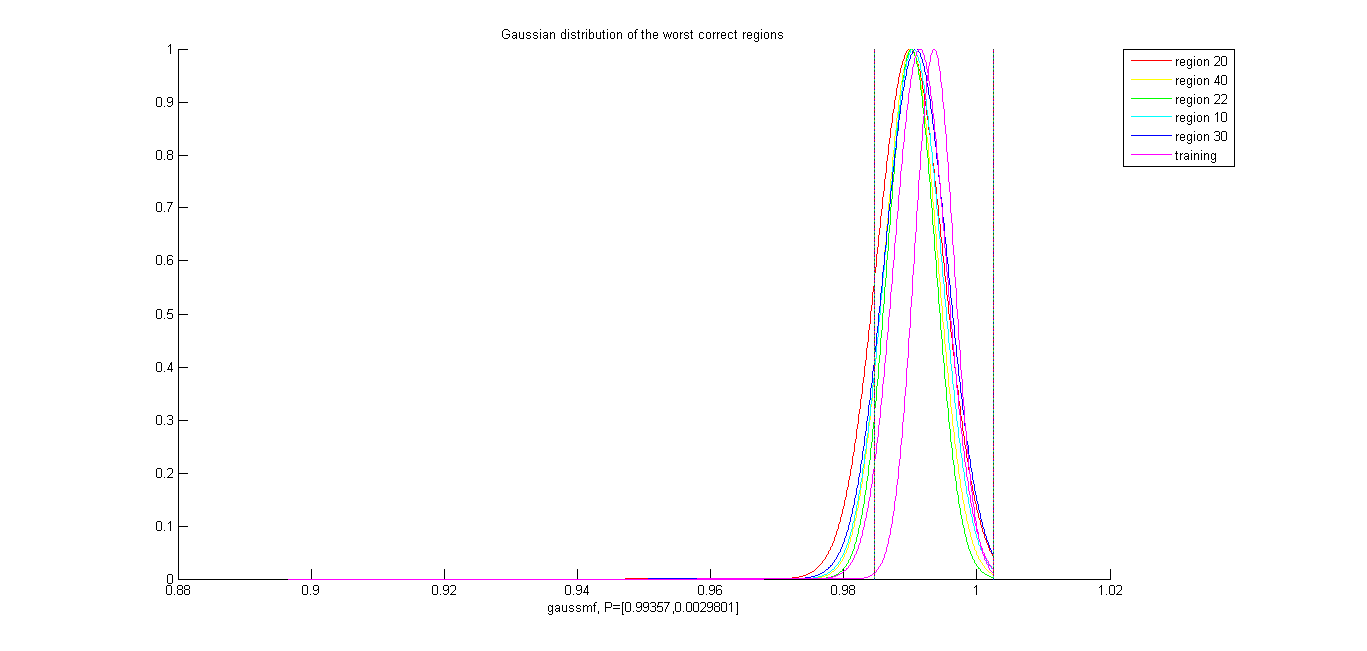
\includegraphics[width=1\textwidth]{img/worst_best_graph}
\caption{ I peggiori tra i migliori }
\label{fig:worstBestGraph}
\end{center}
\end{figure}

I risultati ottenuti in seguito all'applicazione del metodo da noi implementato su un numero significativo di immagini, si sono rivelati soddisfacenti. Infatti nei casi di classificazione di falsi positivi e veri negativi è bastato modificare opportunamente i parametri di configurazione per ottenere una classificazione esatta.

\pagebreak

\addcontentsline{toc}{section}{Acronimi}
\markboth{Elenco degli acronimi}{Elenco degli acronimi}
\section*{Acronimi}

% \ac{IPv6} con questo comando viene scritto per esteso il nome dell'acronimo (output: Internet Protocol Version 6 (IPv6)
% \acf{} come prima
% \acs{} inserisce l'acronimo
% \acl{} inserisce il nome lungo dell'acronimo senza mezionane l'acronimo

\begin{acronym}
\acro {MLBP}{Multi-scale Local Binary Pattern}
\acro {LBP}{Local Binary Pattern}
\end{acronym}
\appendix
\listoffigures    % Indice Figure
\listoftables

\addcontentsline{toc}{section}{Bibliografia}
\bibliographystyle{IEEEtran}
\bibliography{bibliography}

\end{document}

